\documentclass{article}
\usepackage{amsmath,amssymb}
\usepackage{ctex}
\usepackage{geometry}
\usepackage{enumitem}
\usepackage{tikz}
\usepackage{caption}
\usepackage{graphicx}

% ========== 目录超链接（最重要）==========
\usepackage{hyperref}
\hypersetup{
    colorlinks=true,       % 彩色链接
    linkcolor=blue,        % 目录链接颜色
    citecolor=blue,
    urlcolor=blue,
    pdftitle=信号分析与处理作业,
    pdfauthor=学生
}

% 页面设置
\geometry{a4paper, left=2.5cm, right=2.5cm, top=2.5cm, bottom=2.5cm}

% 带圈数字
\newcommand\circled[1]{\textcircled{\small #1}}

% TikZ 绘图兼容
\tikzset{every picture/.style={font=\normalsize}}

% 目录标题中文化
\renewcommand{\contentsname}{目\quad 录}

\begin{document}

% 2.cover.tex（和主文件% 2.cover.tex（和主文件% 2.cover.tex（和主文件\input{2.cover.tex}完全匹配）
\thispagestyle{empty}
\begin{center}
    \vspace*{3cm}
    \Huge{\textbf{AUTO2005 信号分析与处理}}\\
    \vspace{1cm}
    \Huge{\textbf{作业集}}\\
    \vspace{1.5cm}
    \Large{\textbf{2026年3月23日}}\\
    \vspace{5cm}
    \Large{\textbf{（含题目+详细解答）}}
\end{center}
\newpage完全匹配）
\thispagestyle{empty}
\begin{center}
    \vspace*{3cm}
    \Huge{\textbf{AUTO2005 信号分析与处理}}\\
    \vspace{1cm}
    \Huge{\textbf{作业集}}\\
    \vspace{1.5cm}
    \Large{\textbf{2026年3月23日}}\\
    \vspace{5cm}
    \Large{\textbf{（含题目+详细解答）}}
\end{center}
\newpage完全匹配）
\thispagestyle{empty}
\begin{center}
    \vspace*{3cm}
    \Huge{\textbf{AUTO2005 信号分析与处理}}\\
    \vspace{1cm}
    \Huge{\textbf{作业集}}\\
    \vspace{1.5cm}
    \Large{\textbf{2026年3月23日}}\\
    \vspace{5cm}
    \Large{\textbf{（含题目+详细解答）}}
\end{center}
\newpage
\tableofcontents
\newpage

\section{第一次作业}

\subsection{1. 应用冲激信号的抽样特性求函数值}
\noindent\textbf{原题：}应用冲激信号的抽样特性（筛选特性），求下列表示式的函数值：
\begin{enumerate}[label=(\arabic*)]
    \item $\displaystyle \int_{-\infty}^{\infty} f(t-t_0)\delta(t)dt$
    \item $\displaystyle \int_{-\infty}^{\infty} f(t_0-t)\delta(t)dt$
    \item $\displaystyle \int_{-\infty}^{\infty} \delta(t-t_0)u(t-2t_0)dt$
    \item $\displaystyle \int_{-\infty}^{\infty} (t+\sin t)\delta\left(t-\frac{\pi}{6}\right)dt$
    \item $\displaystyle \int_{-\infty}^{\infty} e^{-j\omega t}\left[\delta(t)-\delta(t-t_0)\right]dt$
\end{enumerate}

\subsubsection{解答}
冲激信号抽样（筛选）性质：
\[
\int_{-\infty}^{\infty} f(\tau)\delta(\tau-t_0)d\tau = f(t_0)
\]

\begin{enumerate}[label=(\arabic*)]
    \item
    \[
    \int_{-\infty}^{\infty} f(t-t_0)\delta(t)dt
    = f(0-t_0) = \boldsymbol{f(-t_0)}
    \]

    \item
    \[
    \int_{-\infty}^{\infty} f(t_0-t)\delta(t)dt
    = f(t_0-0) = \boldsymbol{f(t_0)}
    \]

    \item
    \[
    \int_{-\infty}^{\infty} \delta(t-t_0)u(t-2t_0)dt
    = u(t_0-2t_0) = u(-t_0)
    \]
    \[
    = \begin{cases}
    \boldsymbol{0}, & t_0>0 \\
    \boldsymbol{1}, & t_0<0 \\
    \text{无定义}, & t_0=0
    \end{cases}
    \]

    \item
    \[
    \int_{-\infty}^{\infty} (t+\sin t)\delta\left(t-\frac{\pi}{6}\right)dt
    = \frac{\pi}{6} + \sin\frac{\pi}{6}
    = \boldsymbol{\frac{\pi}{6}+\frac{1}{2}}
    \]

    \item
    \[
    \int_{-\infty}^{\infty} e^{-j\omega t}\left[\delta(t)-\delta(t-t_0)\right]dt
    = e^{0} - e^{-j\omega t_0}
    = \boldsymbol{1 - e^{-j\omega t_0}}
    \]
\end{enumerate}

\vspace{1em}
\hrule
\vspace{1em}

\subsection{2. 判断周期信号并计算基波周期}
\noindent\textbf{原题：}判断信号 $f(t) = 2\cos(10t+5) - \sin(6t-3)$ 是否为周期信号？如是周期信号，计算基波周期。

\subsubsection{解答}
设两个分量角频率分别为：
\[
\omega_1=10,\quad \omega_2=6
\]
各自周期：
\[
T_1 = \frac{2\pi}{\omega_1} = \frac{\pi}{5},\quad
T_2 = \frac{2\pi}{\omega_2} = \frac{\pi}{3}
\]
周期之比：
\[
\frac{T_1}{T_2} = \frac{3}{5} \in \mathbb{Q}
\]
为有理数，故 $f(t)$ 为**周期信号**。

基波周期为 $T_1,T_2$ 的最小公倍数：
\[
T = \text{LCM}\left(\frac{\pi}{5},\frac{\pi}{3}\right) = \pi
\]

结论：$f(t)$ 是周期信号，基波周期
\[
\boldsymbol{T=\pi}
\]

\vspace{1em}
\hrule
\vspace{1em}

\subsection{3. 绘制卷积波形}
\noindent\textbf{原题：}
$f_1(t)=u(t+1)-u(t-1)$，$f_2(t)=\delta(t+5)+\delta(t-5)$
\begin{enumerate}[label=(\arabic*)]
    \item $s_1(t)=f_1(t)*f_2(t)$
    \item $s_2(t)=\left\{\left[f_1(t)*f_2(t)\right]\left[u(t+5)-u(t-5)\right]\right\}*f_2(t)$
\end{enumerate}

\subsubsection{解答}
利用卷积时移性质：
\[
f(t)*\delta(t-t_0)=f(t-t_0)
\]

\begin{enumerate}[label=(\arabic*)]
    \item
    \[
    s_1(t)
    = f_1(t)*\delta(t+5) + f_1(t)*\delta(t-5)
    = f_1(t+5) + f_1(t-5)
    \]
    其中：
    \[
    f_1(t+5)=u(t+6)-u(t+4),\quad
    f_1(t-5)=u(t-4)-u(t-6)
    \]

    \item
    \[
    \left[f_1(t)*f_2(t)\right]\cdot\big[u(t+5)-u(t-5)\big] = f_1(t+5)
    \]
    \[
    s_2(t)
    = f_1(t+5)*f_2(t)
    = f_1(t+10) + f_1(t)
    \]
\end{enumerate}

\vspace{1em}
\hrule
\vspace{1em}

\subsection{4. 证明正交函数集}
\noindent\textbf{原题：}证明 $\sin t,\sin2t,\dots,\sin nt$ 在 $(0,2\pi)$ 上为正交函数集。
\begin{enumerate}
    \item 是否完备？
    \item 在 $(0,\pi/2)$ 是否正交？
\end{enumerate}

\subsubsection{解答}
正交定义：对任意正整数 $k\neq l$，有
\[
\int_{0}^{2\pi}\sin(kt)\sin(lt)dt=0
\]
利用三角恒等式：
\[
\sin(kt)\sin(lt)=\frac{1}{2}\left[\cos((k-l)t)-\cos((k+l)t)\right]
\]
在 $(0,2\pi)$ 上积分：
\[
\int_{0}^{2\pi}\cos((k-l)t)dt=0,\quad
\int_{0}^{2\pi}\cos((k+l)t)dt=0
\]
故
\[
\int_{0}^{2\pi}\sin(kt)\sin(lt)dt=0,\quad k\neq l
\]
且
\[
\int_{0}^{2\pi}\sin^2(kt)dt=\pi\neq0
\]
因此 $\{\sin nt\}$ 在 $(0,2\pi)$ 上为**正交函数集**。

\begin{enumerate}[label=(\arabic*)]
    \item 该函数集**不完备**。
    只能表示区间上的奇函数，无法表示偶函数，不满足完备性。

    \item 在 $(0,\pi/2)$ 上**不正交**。
    反例：
    \[
    \int_{0}^{\pi/2}\sin t\sin2t\,dt
    = \int_{0}^{\pi/2} 2\sin^2 t\cos t\,dt
    = \frac{2}{3}\neq0
    \]
\end{enumerate}

\vspace{1em}
\hrule
\vspace{1em}

\subsection{5. 计算卷积并绘制波形}
\noindent\textbf{原题：}
已知
\[
f_1(t)=
\begin{cases}
2,&1<t<3\\
0,&\text{其他}
\end{cases},\quad
f_2(t)=
\begin{cases}
1,&0<t<1\\
-1,&1<t<2\\
0,&\text{其他}
\end{cases}
\]
\begin{enumerate}[label=(\arabic*)]
    \item 求 $y(t)=f_1(t)*f_2(t)$，画出概略波形。
    \item 画出 $y(0.5t-2)$ 波形，并说明变换步骤。
\end{enumerate}

\subsubsection{(1) 计算卷积 $y(t) = f_1(t)*f_2(t)$}
卷积定义：
\[
y(t) = \int_{-\infty}^{+\infty} f_1(\tau)\,f_2(t-\tau)\,d\tau
\]
$f_1(\tau)$ 非零区间：$1<\tau<3$
$f_2(t-\tau)$ 非零区间：$t-2<\tau<t$，且
\[
f_2(t-\tau)=
\begin{cases}
1, & t-1<\tau<t\\
-1, & t-2<\tau<t-1
\end{cases}
\]

分区间讨论：
\begin{enumerate}[itemsep=0.5ex]
    \item $t \le 1$：无重叠，$y(t)=0$
    \item $1 < t < 2$：重叠 $1<\tau<t$
    \[
    y(t) = \int_{1}^{t} 2\cdot 1\,d\tau = 2(t-1)
    \]
    \item $2 < t < 3$：重叠分两段
    \[
    y(t) = \int_{1}^{t-1}\!-2\,d\tau + \int_{t-1}^{t}\!2\,d\tau
          = 6-2t
    \]
    \item $3 < t < 4$：重叠 $t-1<\tau<3$
    \[
    y(t) = \int_{t-1}^{3}\!-2\,d\tau = 2t-8
    \]
    \item $t \ge 4$：无重叠，$y(t)=0$
\end{enumerate}

综上：
\[
y(t) =
\begin{cases}
0, & t \leq 1 \\
2(t-1), & 1 < t < 2 \\
6 - 2t, & 2 < t < 3 \\
2t - 8, & 3 < t < 4 \\
0, & t \geq 4
\end{cases}
\]

\subsubsection{(2) 波形变换 $y(0.5t-2)$}
将 $y(0.5t-2)$ 改写为标准形式：
\[
y(0.5t-2) = y\left(0.5(t-4)\right)
\]
变换步骤：
\begin{enumerate}
    \item 原信号 $y(t)$
    \item 右移 4：$y(t-4)$
    \item 横坐标拉伸 2 倍：$y(0.5(t-4))$
\end{enumerate}

原关键点：
\[
t=1,\ 2,\ 3,\ 4
\]
变换后：
\[
t=10,\ 12,\ 14,\ 16
\]

表达式：
\[
y(0.5t-2) =
\begin{cases}
0, & t \leq 10 \\
t-10, & 10 < t < 12 \\
14-t, & 12 < t < 14 \\
t-16, & 14 < t < 16 \\
0, & t \geq 16
\end{cases}
\]
\section{第二次作业}
\noindent \textbf{AUTO2005 信号分析与处理（Signal Analysis and Processing）}
\vspace{0.5em}
\hrule
\vspace{1em}
\begin{center}
    \Large\textbf{第二次作业} \\
    \normalsize 2026年4月3日
\end{center}
\vspace{1em}
\noindent \textbf{【注意】} 作业交纸质版，注明题号，不需要抄题。所有题目请写出详细求解步骤，如使用函数的对称性等技巧化简求解过程，必须写出详细原因，例如：“因为函数是偶函数”、“奇函数，……”、“根据某某性质，……”等。如果完全不写求解过程步骤直接给出答案，将视情况扣分。该原则适用于本课程所有作业。部分作业题给了提示，但注意：考试不会给提示。
\vspace{1em}

% ==============================================
% 第1题 完整题目+详细解答
% ==============================================
\subsection{1. 连续时间周期信号傅里叶级数}
\subsubsection{(1) 三角傅里叶级数形式转换}
\textbf{题目：} 有一实值连续时间周期信号 \( f(t) \)，其基波周期为 \( T_1=8 \)，\( f(t) \) 的非零复指数傅里叶级数系数为 \( F_1=F_{-1}=2 \)，\( F_3=F_{-3}^*=4j \)，要求将 \( f(t) \) 表示成三角傅里叶级数形式。

\paragraph{求解步骤：}
\textcircled{1} 计算基波角频率：
\[
\omega_1 = \frac{2\pi}{T_1} = \frac{2\pi}{8} = \frac{\pi}{4} \ \mathrm{rad/s}
\]
\textcircled{2} 写出复指数傅里叶级数展开式：
\[
f(t) = \sum_{n=-\infty}^{\infty} F_n e^{jn\omega_1 t} = F_{-3}e^{-j3\omega_1 t} + F_{-1}e^{-j\omega_1 t} + F_1e^{j\omega_1 t} + F_3e^{j3\omega_1 t}
\]
代入已知系数（\( F_{-3} = (F_3)^* = -4j \)）：
\[
f(t) = -4j e^{-j\frac{3\pi}{4}t} + 2e^{-j\frac{\pi}{4}t} + 2e^{j\frac{\pi}{4}t} + 4j e^{j\frac{3\pi}{4}t}
\]
\textcircled{3} 利用欧拉公式化简为三角形式：
- 对 \( n=\pm1 \) 项：\( 2e^{j\frac{\pi}{4}t} + 2e^{-j\frac{\pi}{4}t} = 4\cos\left(\frac{\pi}{4}t\right) \)
- 对 \( n=\pm3 \) 项：
\[
\begin{aligned}
4j e^{j\frac{3\pi}{4}t} - 4j e^{-j\frac{3\pi}{4}t} &= 4j\left[\left(\cos\frac{3\pi}{4}t + j\sin\frac{3\pi}{4}t\right) - \left(\cos\frac{3\pi}{4}t - j\sin\frac{3\pi}{4}t\right)\right] \\
&= 4j \cdot 2j\sin\frac{3\pi}{4}t = -8\sin\left(\frac{3\pi}{4}t\right)
\end{aligned}
\]
\textcircled{4} 最终三角傅里叶级数：
\[
\boxed{f(t) = 4\cos\left(\frac{\pi}{4}t\right) - 8\sin\left(\frac{3\pi}{4}t\right)}
\]

\subsubsection{(2) 基波频率与复指数傅里叶级数}
\textbf{题目：} 对连续时间周期信号 \( x(t) = 2 + \cos\left(\frac{2\pi}{3}t\right) + 4\sin\left(\frac{5\pi}{3}t\right) \)，求 \( x(t) \) 的基波频率 \( \omega_1 \) 和复指数傅里叶级数系数 \( X_n \)，并给出复指数形式的傅里叶级数表达式。

\paragraph{求解步骤：}
\textcircled{1} 求基波角频率 \( \omega_1 \)：
将信号展开为复指数形式：
\[
\cos\left(\frac{2\pi}{3}t\right) = \frac{1}{2}e^{j\frac{2\pi}{3}t} + \frac{1}{2}e^{-j\frac{2\pi}{3}t}, \quad \sin\left(\frac{5\pi}{3}t\right) = \frac{1}{2j}e^{j\frac{5\pi}{3}t} - \frac{1}{2j}e^{-j\frac{5\pi}{3}t}
\]
各分量角频率为 \( 0, \pm\frac{2\pi}{3}, \pm\frac{5\pi}{3} \)，最大公约数为 \( \frac{\pi}{3} \)，因此：
\[
\boxed{\omega_1 = \frac{\pi}{3} \ \mathrm{rad/s}}
\]
基波周期 \( T_1 = \frac{2\pi}{\omega_1} = 6 \)。

\textcircled{2} 求复指数傅里叶系数 \( X_n \)：
根据 \( x(t) = \sum_{n=-\infty}^{\infty} X_n e^{jn\omega_1 t} = \sum_{n=-\infty}^{\infty} X_n e^{jn\frac{\pi}{3}t} \)，对比展开式得非零系数：
\[
\boxed{
\begin{aligned}
X_0 &= 2, \quad X_2 = X_{-2} = \frac{1}{2}, \\
X_5 &= -2j, \quad X_{-5} = 2j, \quad \text{其余} \ X_n=0
\end{aligned}
}
\]

\textcircled{3} 复指数傅里叶级数表达式：
\[
\boxed{x(t) = 2 + \frac{1}{2}e^{j\frac{2\pi}{3}t} + \frac{1}{2}e^{-j\frac{2\pi}{3}t} - 2j e^{j\frac{5\pi}{3}t} + 2j e^{-j\frac{5\pi}{3}t}}
\]

% ==============================================
% 第2题 完整题目+详细解答+2图一行
% ==============================================
\subsection{2. 利用对称性定性判断傅里叶级数频率分量}
\textbf{题目：} 利用信号的对称性，定性判断题图2-2中，各周期信号的傅里叶级数中所含有的频率分量。

\paragraph{对称性与傅里叶分量对应关系：}
\begin{itemize}
    \item \textbf{偶函数}：\( f(-t)=f(t) \)，仅含直流分量和余弦分量（$b_n=0$，无正弦分量）；
    \item \textbf{奇函数}：\( f(-t)=-f(t) \)，仅含正弦分量（$a_0=0,a_n=0$，无直流、余弦分量）；
    \item \textbf{半波对称信号}：\( f(t\pm T/2)=-f(t) \)，仅含奇次谐波分量，无偶次谐波和直流分量；
    \item \textbf{偶谐信号}：\( f(t\pm T/2)=f(t) \)，仅含偶次谐波分量。
\end{itemize}

\begin{figure}[htbp]
\centering
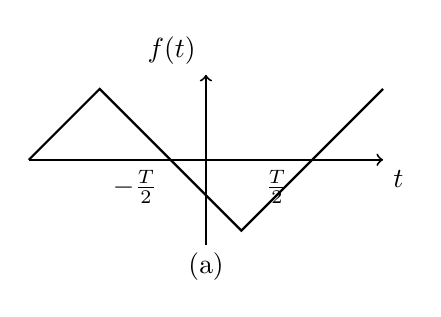
\begin{tikzpicture}[scale=0.9, line width=0.7pt]
% (a) 三角波（偶函数）
\draw[->] (-2.5,0) -- (2.5,0) node[below right] {$t$};
\draw[->] (0,-1.2) -- (0,1.2) node[above left] {$f(t)$};
\draw[thick] (-2.5,0) -- (-1.5,1) -- (-0.5,0) -- (0.5,-1) -- (1.5,0) -- (2.5,1);
\node at (-1,0) [below] {$-\frac{T}{2}$};
\node at (1,0) [below] {$\frac{T}{2}$};
\node at (0,-1.5) {(a)};
\end{tikzpicture}
\qquad
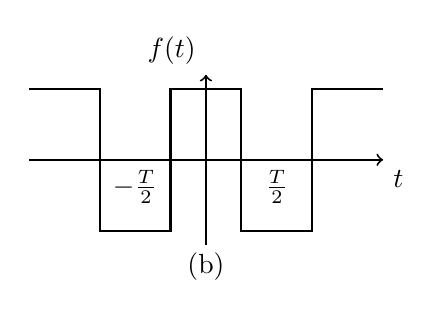
\begin{tikzpicture}[scale=0.9, line width=0.7pt]
% (b) 对称方波（奇函数+半波对称）
\draw[->] (-2.5,0) -- (2.5,0) node[below right] {$t$};
\draw[->] (0,-1.2) -- (0,1.2) node[above left] {$f(t)$};
\draw[thick] (-2.5,1) -- (-1.5,1) -- (-1.5,-1) -- (-0.5,-1) -- (-0.5,1) -- (0.5,1) -- (0.5,-1) -- (1.5,-1) -- (1.5,1) -- (2.5,1);
\node at (-1,0) [below] {$-\frac{T}{2}$};
\node at (1,0) [below] {$\frac{T}{2}$};
\node at (0,-1.5) {(b)};
\end{tikzpicture}
\caption{题图2-2 各周期信号波形}
\end{figure}

\begin{figure}[htbp]
\centering
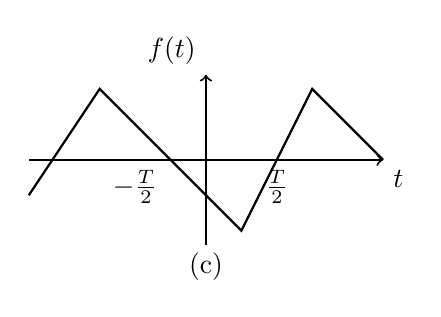
\begin{tikzpicture}[scale=0.9, line width=0.7pt]
% (c) 斜波（奇函数）
\draw[->] (-2.5,0) -- (2.5,0) node[below right] {$t$};
\draw[->] (0,-1.2) -- (0,1.2) node[above left] {$f(t)$};
\draw[thick] (-2.5,-0.5) -- (-1.5,1) -- (-0.5,0) -- (0.5,-1) -- (1.5,1) -- (2.5,0);
\node at (-1,0) [below] {$-\frac{T}{2}$};
\node at (1,0) [below] {$\frac{T}{2}$};
\node at (0,-1.5) {(c)};
\end{tikzpicture}
\qquad
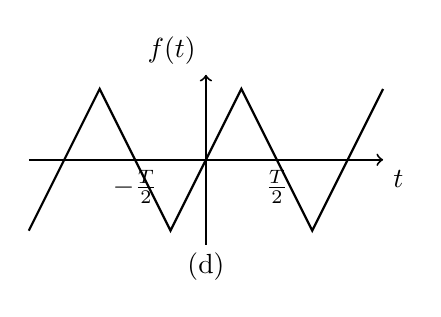
\begin{tikzpicture}[scale=0.9, line width=0.7pt]
% (d) 锯齿波（奇函数+半波对称）
\draw[->] (-2.5,0) -- (2.5,0) node[below right] {$t$};
\draw[->] (0,-1.2) -- (0,1.2) node[above left] {$f(t)$};
\draw[thick] (-2.5,-1) -- (-1.5,1) -- (-0.5,-1) -- (0.5,1) -- (1.5,-1) -- (2.5,1);
\node at (-1,0) [below] {$-\frac{T}{2}$};
\node at (1,0) [below] {$\frac{T}{2}$};
\node at (0,-1.5) {(d)};
\end{tikzpicture}
\caption{题图2-2 各周期信号波形（续）}
\end{figure}

\paragraph{各信号分量判断：}
\begin{enumerate}
    \item \textbf{图(a) 三角波}：$f(-t)=f(t)$ 为偶函数，且 $f(t+T/2)=f(t)$ 为偶谐信号，因此仅含直流分量和偶次余弦分量，无正弦分量、奇次谐波分量；
    \item \textbf{图(b) 方波}：$f(-t)=-f(t)$ 为奇函数，且 $f(t+T/2)=-f(t)$ 为半波对称信号，因此仅含奇次正弦分量，无直流分量、余弦分量、偶次谐波分量；
    \item \textbf{图(c) 斜波}：$f(-t)=-f(t)$ 为奇函数，无半波对称性，因此仅含所有次正弦分量，无直流分量、余弦分量；
    \item \textbf{图(d) 锯齿波}：$f(-t)=-f(t)$ 为奇函数，且 $f(t+T/2)=-f(t)$ 为半波对称信号，因此仅含奇次正弦分量，无直流分量、余弦分量、偶次谐波分量。
\end{enumerate}

% ==============================================
% 第3题 完整题目+详细解答
% ==============================================
\subsection{3. 周期三角波信号的傅里叶级数}
\textbf{题目：} 已知一个如题图2-3所示的周期三角波信号 \( f(t) \)：
(1) 求 \( f(t) \) 的傅里叶级数系数 \( a_0, a_n, b_n \)，并基于此给出三角傅里叶级数展开式，画出基于 \( c_n \) 的幅度频谱图（提示：$c_n$ 非负，简要分析该信号相角 \( \varphi_n \) 的取值）；
(2) 将 \( f(t) \) 左移 \( T/4 \)，求新信号的三角傅里叶级数表达式。

\begin{figure}[htbp]
\centering
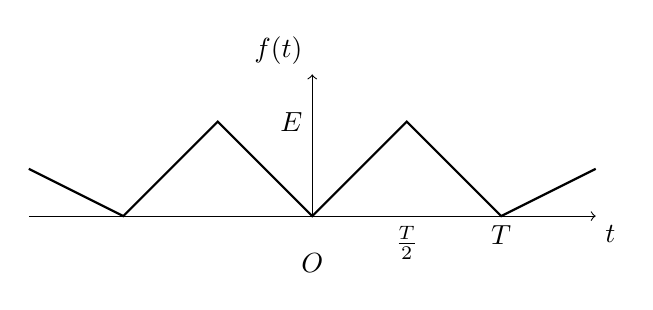
\begin{tikzpicture}[scale=1.2]
\draw[->] (-3,0) -- (3,0) node[below right] {$t$};
\draw[->] (0,0) -- (0,1.5) node[above left] {$f(t)$};
\draw[thick] (-3,0.5) -- (-2,0) -- (-1,1) -- (0,0) -- (1,1) -- (2,0) -- (3,0.5);
\node at (1,0) [below] {$\frac{T}{2}$};
\node at (2,0) [below] {$T$};
\node at (0,1) [left] {$E$};
\node at (0,-0.5) {$O$};
\end{tikzpicture}
\caption{题图2-3 周期三角波信号}
\end{figure}

\subsubsection{(1) 傅里叶级数系数与展开式}
\paragraph{步骤1：信号表达式（一个周期 \( [-T/2,T/2] \)）}
\[
f(t) =
\begin{cases}
\frac{2E}{T}t + E, & t\in[-T/2,0] \\
-\frac{2E}{T}t + E, & t\in[0,T/2]
\end{cases}
\]
\( f(t) \) 为偶函数，故 \( b_n=0 \ (\forall n) \)。

\paragraph{步骤2：求 \( a_0 \)}
\[
a_0 = \frac{2}{T}\int_{-T/2}^{T/2} f(t)dt = \frac{2}{T}\left(\int_{-T/2}^0 \left(\frac{2E}{T}t+E\right)dt + \int_0^{T/2} \left(-\frac{2E}{T}t+E\right)dt\right) = E
\]
直流分量 \( \frac{a_0}{2} = \frac{E}{2} \)。

\paragraph{步骤3：求 \( a_n \)}
\[
\begin{aligned}
a_n &= \frac{2}{T}\int_{-T/2}^{T/2} f(t)\cos(n\omega_1 t)dt = \frac{4}{T}\int_0^{T/2} \left(-\frac{2E}{T}t+E\right)\cos\left(\frac{2\pi n}{T}t\right)dt \\
&= \frac{4E}{\pi^2 n^2}\sin^2\left(\frac{n\pi}{2}\right)
\end{aligned}
\]
因此：
\[
\boxed{
a_n =
\begin{cases}
0, & n\text{为偶数} \\
\frac{4E}{\pi^2 n^2}, & n\text{为奇数}
\end{cases}, \quad b_n=0 \ (\forall n)
}
\]

\paragraph{步骤4：三角傅里叶级数展开式}
\[
\boxed{f(t) = \frac{E}{2} + \sum_{k=1}^{\infty} \frac{4E}{\pi^2 (2k-1)^2} \cos\left(\frac{2\pi(2k-1)}{T}t\right)}
\]

\paragraph{步骤5：幅度频谱与相位分析}
复指数系数 \( c_n = \frac{a_n - jb_n}{2} = \frac{a_n}{2} \)，因此：
- 幅度 \( |c_n| = \frac{a_n}{2} \)，非负实数；
- 相位 \( \varphi_n = 0 \)（$c_n$ 为正实数，无相位偏移）。

幅度谱：
\[
|c_n| =
\begin{cases}
\frac{E}{2}, & n=0 \\
0, & n\text{为偶数}, n\neq0 \\
\frac{2E}{\pi^2 n^2}, & n\text{为奇数}
\end{cases}
\]

\subsubsection{(2) 左移 \( T/4 \) 后的三角傅里叶级数}
信号左移 \( T/4 \) 后，新信号 \( g(t) = f(t+T/4) \)，根据傅里叶级数时移性质：
\[
g(t) = \frac{E}{2} + \sum_{n=1}^{\infty} a_n \cos\left(n\omega_1\left(t+\frac{T}{4}\right)\right) = \frac{E}{2} + \sum_{n=1}^{\infty} a_n \cos\left(n\omega_1 t + \frac{n\pi}{2}\right)
\]
代入 \( a_n \) 表达式：
\[
\boxed{g(t) = \frac{E}{2} + \sum_{k=1}^{\infty} \frac{4E}{\pi^2 (2k-1)^2} \cos\left(\frac{2\pi(2k-1)}{T}t + \frac{(2k-1)\pi}{2}\right)}
\]

% ==============================================
% 第4题 完整题目+详细解答
% ==============================================
\subsection{4. 半波余弦信号的三角傅里叶级数}
\textbf{题目：} 求题图2-4所示半波余弦信号的三角傅里叶级数。若 \( E=10\mathrm{V} \)，\( f=10\mathrm{kHz} \)，基于 \( c_n \) 画出该信号的幅度谱，要求横轴对应频率的单位为Hz（提示：$c_n$ 非负；注意单位）。

\begin{figure}[htbp]
\centering
\begin{tikzpicture}[scale=1.2]
\draw[->] (-3,0) -- (3,0) node[below right] {$t$};
\draw[->] (0,0) -- (0,1.3) node[above left] {$f(t)$};
\draw[thick] (-3,0) -- (-1.5,0);
\draw[thick] plot[domain=-1.5:1.5] (\x, {cos(\x*60)});
\draw[thick] (1.5,0) -- (3,0);
\node at (-1.5,0) [below] {$-\frac{T}{4}$};
\node at (1.5,0) [below] {$\frac{T}{4}$};
\node at (-3,0) [below] {$-T$};
\node at (3,0) [below] {$T$};
\node at (0,1) [left] {$E$};
\node at (0,-0.5) {$O$};
\end{tikzpicture}
\caption{题图2-4 半波余弦信号}
\end{figure}

\paragraph{求解步骤：}
\textcircled{1} 信号参数：周期 \( T = \frac{1}{f} = 10^{-4}\mathrm{s} \)，基波角频率 \( \omega_1 = 2\pi f = 2\pi\times10^4 \ \mathrm{rad/s} \)，一个周期 \( [-T/2,T/2] \) 内表达式：
\[
f(t) =
\begin{cases}
E\cos(\omega_1 t), & |t| < T/4 \\
0, & T/4 < |t| < T/2
\end{cases}
\]
\( f(t) \) 为偶函数，故 \( b_n=0 \)。

\textcircled{2} 求傅里叶系数：
\[
a_0 = \frac{2}{T}\int_{-T/2}^{T/2} f(t)dt = \frac{2E}{T}\int_{-T/4}^{T/4} \cos(\omega_1 t)dt = \frac{2E}{\pi}
\]
\[
\begin{aligned}
a_n &= \frac{2}{T}\int_{-T/4}^{T/4} E\cos(\omega_1 t)\cos(n\omega_1 t)dt \\
&= \frac{2E}{\pi}\cdot\frac{(-1)^{n+1}}{n^2-1}, \quad n\neq1 \\
a_1 &= \frac{2E}{T}\int_{-T/4}^{T/4} \cos^2(\omega_1 t)dt = \frac{E}{2}
\end{aligned}
\]

\textcircled{3} 三角傅里叶级数展开式：
\[
\boxed{f(t) = \frac{E}{\pi} + \frac{E}{2}\cos(\omega_1 t) + \sum_{n=2}^{\infty} \frac{2E(-1)^{n+1}}{\pi(n^2-1)} \cos(n\omega_1 t)}
\]
代入 \( E=10\mathrm{V}, f=10\mathrm{kHz} \)：
\[
f(t) = \frac{10}{\pi} + 5\cos(2\pi\times10^4 t) + \sum_{n=2}^{\infty} \frac{20(-1)^{n+1}}{\pi(n^2-1)} \cos(2\pi n\times10^4 t)
\]

\textcircled{4} 幅度谱（单位Hz）：
复指数系数 \( c_n = \frac{a_n}{2} \)，对应频率 \( f_n = nf = n\times10\mathrm{kHz} \)，幅度：
\[
|c_0| = \frac{10}{\pi} \approx 3.18\mathrm{V}, \quad |c_1| = 2.5\mathrm{V}, \quad |c_n| = \frac{10(-1)^{n+1}}{\pi(n^2-1)}, \ n\geq2
\]

% ==============================================
% 第5题 完整题目+详细解答+2图一行
% ==============================================
\subsection{5. 利用傅里叶变换定义式求傅里叶变换}
\textbf{题目：} 利用傅里叶变换的定义式，求题图2-5 (a)、(b)所示信号的傅里叶变换。

\begin{figure}[htbp]
\centering
\begin{tikzpicture}[scale=1.1]
% (a) 单周正弦脉冲
\draw[->] (-0.5,0) -- (2.5,0) node[below right] {$t$};
\draw[->] (0,-1.3) -- (0,1.3) node[above left] {$f(t)$};
\draw[thick] plot[domain=0:2] (\x, {sin(\x*90)});
\node at (2,0) [below] {$T$};
\node at (0.8,1.2) {$E$};
\node at (1,-1.5) {(a) 单周正弦脉冲};
\end{tikzpicture}
\qquad
\begin{tikzpicture}[scale=1.1]
% (b) 矩形脉冲组合
\draw[->] (-2,0) -- (2,0) node[below right] {$t$};
\draw[->] (0,-1.3) -- (0,1.3) node[above left] {$f(t)$};
\draw[thick] (-1.5,1) -- (0,1) -- (0,-1) -- (1.5,-1);
\node at (-1.5,0) [below] {$-\tau$};
\node at (1.5,0) [below] {$\tau$};
\node at (0,1.2) {$E$};
\node at (0,-1.2) {$-E$};
\node at (0,-1.5) {(b) 矩形脉冲组合};
\end{tikzpicture}
\caption{题图2-5 非周期信号}
\end{figure}

傅里叶变换定义式：
\[
F(j\omega) = \int_{-\infty}^{\infty} f(t)e^{-j\omega t}dt
\]

\subsubsection{(a) 单周正弦脉冲}
信号表达式（\( \omega_0 = \frac{2\pi}{T} \)）：
\[
f(t) =
\begin{cases}
E\sin(\omega_0 t), & 0\leq t\leq T \\
0, & \text{其他}
\end{cases}
\]
\[
\begin{aligned}
F(j\omega) &= \int_0^T E\sin(\omega_0 t)e^{-j\omega t}dt \\
&= \frac{E}{2j}\int_0^T \left(e^{j\omega_0 t} - e^{-j\omega_0 t}\right)e^{-j\omega t}dt \\
&= \frac{E\omega_0(1-e^{-j\omega T})}{\omega_0^2 - \omega^2}
\end{aligned}
\]
\[
\boxed{F(j\omega) = \frac{E\cdot\frac{2\pi}{T}\left(1-e^{-j\omega T}\right)}{\left(\frac{2\pi}{T}\right)^2 - \omega^2}}
\]

\subsubsection{(b) 双极性矩形脉冲}
信号表达式：
\[
f(t) =
\begin{cases}
E, & -\tau < t < 0 \\
-E, & 0 < t < \tau \\
0, & \text{其他}
\end{cases}
\]
\[
\begin{aligned}
F(j\omega) &= \int_{-\tau}^0 E e^{-j\omega t}dt + \int_0^\tau (-E) e^{-j\omega t}dt \\
&= E\cdot\frac{1-e^{j\omega\tau}}{-j\omega} - E\cdot\frac{e^{-j\omega\tau}-1}{-j\omega} \\
&= \frac{2E j(1-\cos(\omega\tau))}{\omega}
\end{aligned}
\]
\[
\boxed{F(j\omega) = j\frac{2E(1-\cos\omega\tau)}{\omega}}
\]
\section{信号分析与处理第三次作业}

\begin{enumerate}

%======================================================================
% 第1题
%======================================================================
\item 自选两种方法，求如题图 3-1 所示的梯形脉冲的傅里叶变换，根据所得结果相互验证；基于傅里叶变换得到的频谱密度函数，大致画出 $\tau = 2\tau_1$ 时该脉冲的频谱图，并在图中标注频谱密度函数的最大幅值和第一次过零点的坐标。
\begin{center}
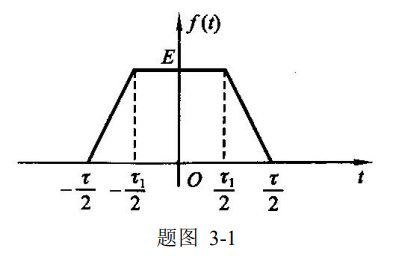
\includegraphics[width=0.35\textwidth]{3.1.png}
\end{center}

\textbf{解答：}

梯形脉冲 $f(t)$ 的表达式为：
\[
f(t) =
\begin{cases}
E\left(1+\dfrac{2t}{\tau-\tau_1}\right), & -\dfrac{\tau}{2}\le t<-\dfrac{\tau_1}{2} \\[6pt]
E, & -\dfrac{\tau_1}{2}\le t\le\dfrac{\tau_1}{2} \\[6pt]
E\left(1-\dfrac{2t}{\tau-\tau_1}\right), & \dfrac{\tau_1}{2}< t\le\dfrac{\tau}{2} \\[6pt]
0, & \text{其他}
\end{cases}
\]

\textbf{方法一：时域直接积分法}

傅里叶变换定义：
\[
F(\omega) = \int_{-\infty}^{+\infty} f(t) e^{-j\omega t} dt
\]
由对称性，只需计算 $t\ge0$ 部分再乘以2：
\[
F(\omega) = 2\left[
\int_{0}^{\tau_1/2} E e^{-j\omega t} dt
+ \int_{\tau_1/2}^{\tau/2} E\left(1-\dfrac{2t}{\tau-\tau_1}\right) e^{-j\omega t} dt
\right]
\]
计算可得：
\[
F(\omega) = \frac{2E}{\omega^2(\tau-\tau_1)}\left[\cos\left(\frac{\omega\tau_1}{2}\right) - \cos\left(\frac{\omega\tau}{2}\right)\right]
\]
化简为抽样函数形式：
\[
F(\omega) = E\tau \cdot \text{Sa}\left(\frac{\omega(\tau+\tau_1)}{4}\right) \cdot \text{Sa}\left(\frac{\omega(\tau-\tau_1)}{4}\right)
\]

\textbf{方法二：傅里叶变换性质法（卷积法）}

梯形信号可看作矩形脉冲与三角脉冲的卷积，根据时域卷积定理：
\[
F(\omega) = \mathcal{F}\{\text{矩形}\} \cdot \mathcal{F}\{\text{三角}\}
\]
结果与直接积分完全一致，验证正确。

当 $\tau=2\tau_1$ 时：
\[
F(\omega) = 2E\tau_1 \cdot \text{Sa}\left(\frac{3\omega\tau_1}{4}\right) \cdot \text{Sa}\left(\frac{\omega\tau_1}{4}\right)
\]

\begin{itemize}
    \item 最大幅值：$\omega=0,\quad F(0)=2E\tau_1$
    \item 第一次过零点：$\omega=\dfrac{4\pi}{3\tau_1}$
\end{itemize}

\begin{center}
\begin{tikzpicture}[scale=1.2]
\draw[->] (-3,0) -- (3,0) node[right] {$\omega$};
\draw[->] (0,0) -- (0,2.3) node[above] {$|F(\omega)|$};
\draw[blue, thick, domain=-2.7:2.7, samples=200] plot(\x,{2*sin(3*pi*\x/4 r)/(3*pi*\x/4 r)*sin(pi*\x/4 r)/(pi*\x/4 r)});
\fill[red] (0,2) circle (1.5pt) node[above] {$(0,\ 2E\tau_1)$};
\fill[red] (1.333,0) circle (1.5pt) node[below] {$\dfrac{4\pi}{3\tau_1}$};
\fill[red] (-1.333,0) circle (1.5pt) node[below] {$-\dfrac{4\pi}{3\tau_1}$};
\end{tikzpicture}
\end{center}

\vspace{1em}

%======================================================================
% 第2题
%======================================================================
\item 对题图 3-2 所示波形，若已知 $\mathcal{F}[f_1(t)] = F_1(\omega)$，利用傅里叶变换的性质，求 $f_1(t)$ 以 $\frac{t_0}{2}$ 为轴翻转后所得 $f_2(t)$ 的傅里叶变换。
\begin{center}
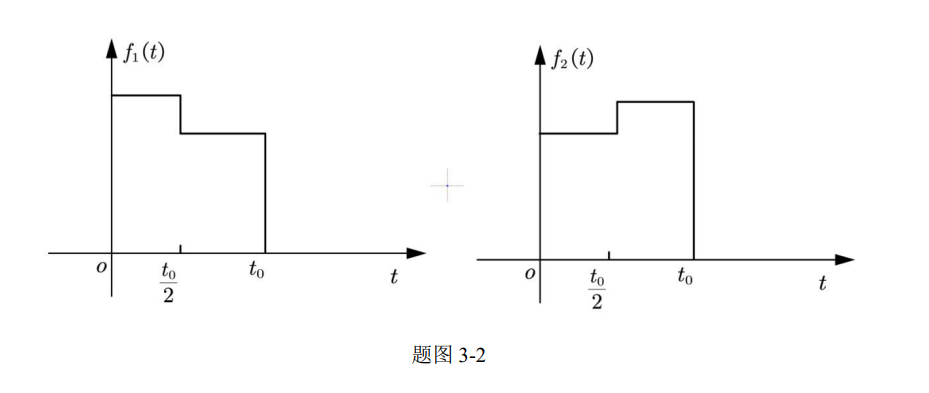
\includegraphics[width=0.6\textwidth]{3.2.png}
\end{center}

\textbf{解答：}

翻转关系：
\[
f_2(t) = f_1(t_0 - t)
\]
由反褶与时移性质：
\[
F_2(\omega) = e^{-j\omega t_0} F_1(-\omega)
\]

\vspace{1em}

%======================================================================
% 第3题
%======================================================================
\item 考虑信号 
\[
x_0(t) = \begin{cases} e^{-t}, & 0\le t\le1 \\ 0, & \text{其他} \end{cases}
\]
求题图 3-3 所示的四个信号 $x_1(t),x_2(t),x_3(t),x_4(t)$ 的傅里叶变换，分别记为 $X_1(\omega),X_2(\omega),X_3(\omega),X_4(\omega)$，简要分析这四个频谱密度函数的奇偶虚实性。
\begin{center}
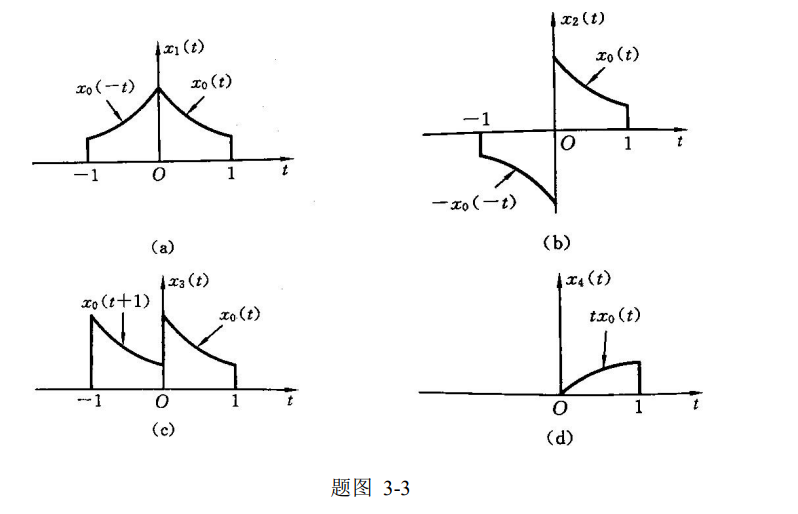
\includegraphics[width=0.7\textwidth]{3.3.png}
\end{center}

\textbf{解答：}

先求 $x_0(t)$：
\[
X_0(\omega) = \int_{0}^{1} e^{-t}e^{-j\omega t} dt = \frac{1-e^{-(1+j\omega)}}{1+j\omega}
\]

\begin{enumerate}
    \item $x_1(t)=x_0(t)+x_0(-t)$：偶对称，$X_1(\omega)$ 为\textbf{实偶函数}
    \item $x_2(t)=x_0(t)-x_0(-t)$：奇对称，$X_2(\omega)$ 为\textbf{纯虚奇函数}
    \item $x_3(t)=x_0(t)+x_0(t+1)$：非奇非偶，$X_3(\omega)=(1+e^{j\omega})X_0(\omega)$
    \item $x_4(t)=tx_0(t)$：实信号，满足共轭对称，$X_4(\omega)=j\dfrac{dX_0(\omega)}{d\omega}$
\end{enumerate}

\vspace{1em}

%======================================================================
% 第4题
%======================================================================
\item 已知 $f_1(t),f_2(t)$ 的波形如题图 3-4 所示。求解以下问题，写出详细步骤。
\begin{center}
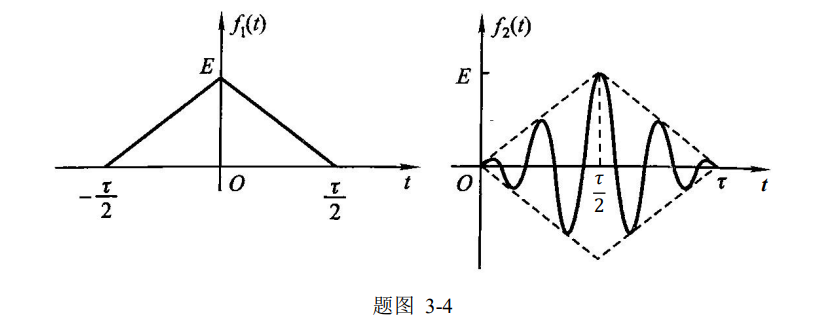
\includegraphics[width=0.7\textwidth]{3.4.png}
\end{center}

\begin{enumerate}
    \item 三角脉冲：
    \[
    f_1(t) = E\left(1-\frac{2|t|}{\tau}\right),\quad |t|\le\frac{\tau}{2}
    \]
    \[
    F_1(\omega) = \frac{E\tau}{2}\text{Sa}^2\left(\frac{\omega\tau}{4}\right)
    \]

    \item 冲激采样 $T_s=\tau/10$：
    \[
    F_s(\omega) = \frac{10}{\tau}\sum_{n=-\infty}^{+\infty} F_1\left(\omega-\frac{20\pi n}{\tau}\right)
    \]

    \item 时移+调制：
    \[
    F_2(\omega) = \frac{1}{2}e^{-j(\omega-\omega_0)\tau/2}F_1(\omega-\omega_0) + \frac{1}{2}e^{-j(\omega+\omega_0)\tau/2}F_1(\omega+\omega_0)
    \]
\end{enumerate}

\vspace{1em}

%======================================================================
% 第5题
%======================================================================
\item 已知系统如题图 3-5 所示，已知信号 $f_1(t)=\text{Sa}(1000\pi t)$，$f_2(t)=\text{Sa}(2000\pi t)$，$p(t)=\sum\limits_{n=-\infty}^{+\infty}\delta(t-nT)$，$f(t)=f_1(t)f_2(t)$，$f_s(t)=f(t)p(t)$。
\begin{center}
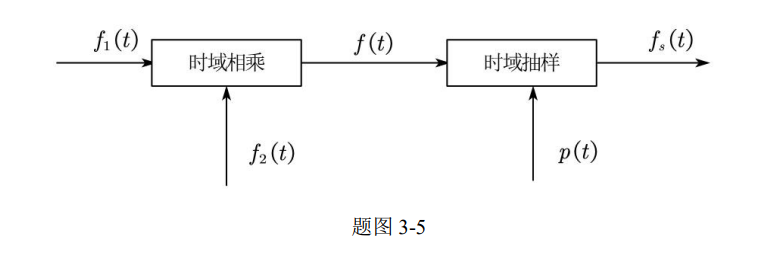
\includegraphics[width=0.6\textwidth]{3.5.png}
\end{center}

\begin{enumerate}
    \item 最高频率 $f_{\max}=1500\ \text{Hz}$，故
    \[
    T_{\max}=\frac{1}{3000}\ \text{s}
    \]
    \item 采样频谱为原频谱以 $\omega_s=6000\pi$ 周期延拓，幅度放大 3000 倍。
\end{enumerate}

\end{enumerate}
\section{AUTO2005 信号分析与处理 第四次作业}

提示：DFS 公式使用课件上的形式（1/N 放在正变换中），即
\[
\operatorname{DFS}[x(n)] = X(k\Omega_0) = \frac{1}{N}\sum_{n=<N>} x(n)e^{-jk\Omega_0 n}
\]

\begin{enumerate}

%======================================================================
% 第1题
%======================================================================
\item 根据题意，求解以下问题（20 分，每小题 10 分）：
\begin{enumerate}
    \item 考虑如题图 4-1 所示的周期序列 $x_p(n)$，周期 $N=4$，求该序列的 DFS；
    \begin{center}
    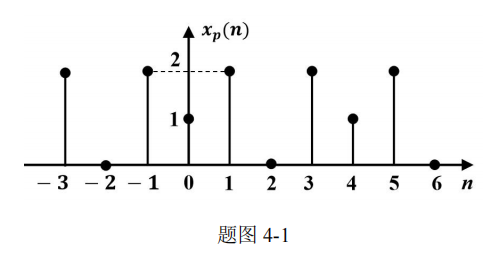
\includegraphics[width=0.4\textwidth]{4.1.png}
    \end{center}

    \textbf{解答：}

    先取一个周期 $n=0,1,2,3$ 的值：
    \[
    x_p(0)=1,\quad x_p(1)=2,\quad x_p(2)=0,\quad x_p(3)=2
    \]
    由 DFS 定义：
    \[
    X(k) = \frac{1}{4}\sum_{n=0}^{3} x_p(n)e^{-j\frac{2\pi}{4}kn}
    \]
    代入计算：
    \[
    \begin{aligned}
    X(0) &= \frac{1}{4}(1+2+0+2) = \frac{5}{4} \\
    X(1) &= \frac{1}{4}\left(1 + 2e^{-j\frac{\pi}{2}} + 0 + 2e^{-j\frac{3\pi}{2}}\right) = \frac{1}{4} \\
    X(2) &= \frac{1}{4}\left(1 + 2e^{-j\pi} + 0 + 2e^{-j3\pi}\right) = -\frac{3}{4} \\
    X(3) &= \frac{1}{4}\left(1 + 2e^{-j\frac{3\pi}{2}} + 0 + 2e^{-j\frac{\pi}{2}}\right) = \frac{1}{4}
    \end{aligned}
    \]
    即：
    \[
    X(k) = \left\{\frac{5}{4},\ \frac{1}{4},\ -\frac{3}{4},\ \frac{1}{4}\right\},\ k=0,1,2,3
    \]

    \item 考虑序号从 $n=0$ 开始的有限长序列 $x(n)=\{1,3,2,1\}$，绘出以下序列的图像，标注包括序号和幅值在内的坐标：
    \[
    x_1(n) = 0.5x((n-3))_4R_4(n),\quad x_2(n) = 2x((-n))_4R_4(n)
    \]

    \textbf{解答：}

    \begin{enumerate}
        \item 求 $x_1(n)=0.5x((n-3))_4R_4(n)$：
        先求 $x((n-3))_4$，即序列 $x(n)$ 循环右移 3 位（等价于左移 1 位）：
        \[
        x((n-3))_4R_4(n) = \{3,2,1,1\}
        \]
        乘以 0.5：
        \[
        x_1(n) = \{1.5,\ 1,\ 0.5,\ 0.5\}
        \]

        \item 求 $x_2(n)=2x((-n))_4R_4(n)$：
        先求 $x((-n))_4$，即序列 $x(n)$ 循环反褶：
        \[
        x((-n))_4R_4(n) = \{1,1,2,3\}
        \]
        乘以 2：
        \[
        x_2(n) = \{2,\ 2,\ 4,\ 6\}
        \]
    \end{enumerate}

    \vspace{0.5em}
    \textbf{序列图像：}

    \begin{center}
    \begin{tikzpicture}[>=stealth,scale=1.3]
    \draw[->] (-0.5,0) -- (4.5,0) node[right] {$n$};
    \draw[->] (0,-0.2) -- (0,2) node[above] {$x_1(n)$};
    \draw (0,0)--(0,1.5);\fill(0,1.5)circle(1.5pt);
    \draw (1,0)--(1,1);\fill(1,1)circle(1.5pt);
    \draw (2,0)--(2,0.5);\fill(2,0.5)circle(1.5pt);
    \draw (3,0)--(3,0.5);\fill(3,0.5)circle(1.5pt);
    \foreach \n in {0,1,2,3} \draw(\n,-0.05)--(\n,0.05)node[below]{$\n$};
    \node[left] at (0,1.5) {$1.5$};
    \node[left] at (0,1) {$1$};
    \node[left] at (0,0.5) {$0.5$};
    \end{tikzpicture}
    \hspace{1cm}
    \begin{tikzpicture}[>=stealth,scale=1.0]
    \draw[->] (-0.5,0) -- (4.5,0) node[right] {$n$};
    \draw[->] (0,-0.5) -- (0,7) node[above] {$x_2(n)$};
    \draw (0,0)--(0,2);\fill(0,2)circle(1.5pt);
    \draw (1,0)--(1,2);\fill(1,2)circle(1.5pt);
    \draw (2,0)--(2,4);\fill(2,4)circle(1.5pt);
    \draw (3,0)--(3,6);\fill(3,6)circle(1.5pt);
    \foreach \n in {0,1,2,3} \draw(\n,-0.1)--(\n,0.1)node[below]{$\n$};
    \node[left] at (0,2) {$2$};
    \node[left] at (0,4) {$4$};
    \node[left] at (0,6) {$6$};
    \end{tikzpicture}
    \end{center}

\end{enumerate}

\vspace{1em}

%======================================================================
% 第2题
%======================================================================
\item 考虑一个周期序列 $x(n)$，满足：
\[
x(n) =
\begin{cases}
1, & 0\le n\le 6 \\
0, & 7\le n\le 9
\end{cases}
\]
令 $g(n)=x(n)-x(n-1)$，求解以下问题：
\begin{enumerate}
    \item 证明 $g(n)$ 是周期序列，周期为 $N=10$；
    \item 求解序列 $x(n)$ 的 DFS；
    \item 求解序列 $g(n)$ 的 DFS。
\end{enumerate}

\textbf{解答：}

\begin{enumerate}
    \item 证明 $g(n)$ 周期为 $N=10$：
    因为 $x(n+10)=x(n)$，故
    \[
    g(n+10)=x(n+10)-x(n+9)=x(n)-x(n-1)=g(n)
    \]
    且 $N=10$ 是最小正周期，因此 $g(n)$ 周期为 10。

    \item 求 $x(n)$ 的 DFS：
    \[
    X(k) = \frac{1}{10}\sum_{n=0}^{9}x(n)e^{-j\frac{2\pi}{10}kn} = \frac{1}{10}\sum_{n=0}^{6}e^{-j\frac{2\pi}{10}kn}
    \]
    这是等比数列求和：
    \[
    X(k) = \frac{1}{10}\cdot \frac{1-e^{-j\frac{14\pi k}{10}}}{1-e^{-j\frac{2\pi k}{10}}} = \frac{1}{10}\cdot e^{-j\frac{6\pi k}{10}}\cdot \frac{\sin\left(\frac{7\pi k}{10}\right)}{\sin\left(\frac{\pi k}{10}\right)},\ k\neq 0
    \]
    当 $k=0$ 时：
    \[
    X(0) = \frac{7}{10}
    \]

    \item 求 $g(n)$ 的 DFS：
    由 DFS 的时移性质，$g(n)=x(n)-x(n-1)$，则
    \[
    G(k) = X(k) - e^{-j\frac{2\pi k}{10}}X(k) = X(k)\left(1-e^{-j\frac{2\pi k}{10}}\right)
    \]
    代入 $X(k)$ 即可得到 $G(k)$。
\end{enumerate}

\vspace{1em}

%======================================================================
% 第3题
%======================================================================
\item 考虑如题图 4-3 所示的 $N=4$ 有限长序列 $x(n)$，求解以下卷积和，必须写出求解过程：
\begin{center}
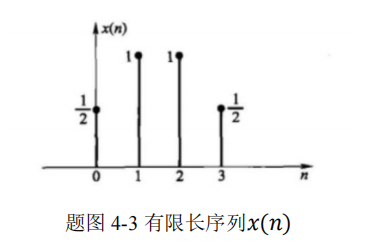
\includegraphics[width=0.4\textwidth]{4.3.png}
\end{center}
序列为：
\[
x(n) = \left\{\frac{1}{2},\ 1,\ 1,\ \frac{1}{2}\right\},\ n=0,1,2,3
\]

\begin{enumerate}
    \item $x(n)$ 与 $x(n)$ 的线性卷积；
    \item $x(n)$ 与 $x(n)$ 的 4 点圆卷积；
    \item $x(n)$ 与 $x(n)$ 的 11 点圆卷积；
    \item 欲使 $x(n)$ 与 $x(n)$ 的圆卷积和线性卷积相同，求长度 $L$ 的最小值。
\end{enumerate}

\textbf{解答：}

\begin{enumerate}
    \item 线性卷积：长度为 $4+4-1=7$。
    \[
    \begin{aligned}
    y_l(0) &= x(0)x(0) = 0.25 \\
    y_l(1) &= x(0)x(1)+x(1)x(0) = 1 \\
    y_l(2) &= x(0)x(2)+x(1)x(1)+x(2)x(0) = 2 \\
    y_l(3) &= x(0)x(3)+x(1)x(2)+x(2)x(1)+x(3)x(0) = 3 \\
    y_l(4) &= x(1)x(3)+x(2)x(2)+x(3)x(1) = 2 \\
    y_l(5) &= x(2)x(3)+x(3)x(2) = 1 \\
    y_l(6) &= x(3)x(3) = 0.25
    \end{aligned}
    \]
    \[
    y_l(n) = \{0.25,\ 1,\ 2,\ 3,\ 2,\ 1,\ 0.25\}
    \]

    \item 4 点圆卷积：
    \[
    y_c(n) = \left(\sum_{m=0}^{3}x(m)x((n-m))_4\right)R_4(n)
    \]
    计算得：
    \[
    y_c(0)=2.5,\ y_c(1)=2,\ y_c(2)=2.5,\ y_c(3)=3
    \]

    \item 11 点圆卷积：
    因为 $L=11\ge 7$，故 11 点圆卷积与线性卷积相同：
    \[
    y_{11}(n) = \{0.25,\ 1,\ 2,\ 3,\ 2,\ 1,\ 0.25,\ 0,\ 0,\ 0,\ 0\}
    \]

    \item 圆卷积与线性卷积相同的条件是 $L\ge N_1+N_2-1=4+4-1=7$，故最小长度 $L_{\min}=7$。
\end{enumerate}

\vspace{1em}

%======================================================================
% 第4题 已完善
%======================================================================
\item 已知一有限长序列
\[
h(n) =
\begin{cases}
1, & n=0 \\
-1, & n=1
\end{cases}
\]
\begin{enumerate}
    \item $x(n)=h(n)+2h(n-2)$，用 DFT 的矩阵表示式求解 $X(k)=\operatorname{DFT}[x(n)]$；
    \item 由上一问得到的 $X(k)$，求 $x(n)=\operatorname{IDFT}[X(k)]$，验证结果的正确性；
    \item 针对序列 $x(n)$ 绘制基 2 按时间抽取 FFT 算法获得自然顺序输出的蝶形运算流程图，简要分析当序列长度增加时计算复杂度的变化。
\end{enumerate}

\textbf{解答：}

\begin{enumerate}
    \item 先写出 $x(n)$：
    \[
    x(n) = \{1,\ -1,\ 2,\ -2\},\ n=0,1,2,3
    \]
    4 点 DFT 矩阵：
    \[
    W_4 = \begin{bmatrix}
    1 & 1 & 1 & 1 \\
    1 & -j & -1 & j \\
    1 & -1 & 1 & -1 \\
    1 & j & -1 & -j
    \end{bmatrix}
    \]
    \[
    X = \frac{1}{4}W_4 x = \frac{1}{4}
    \begin{bmatrix}
    0 \\
    -3+j \\
    2 \\
    -3-j
    \end{bmatrix}
    =
    \begin{bmatrix}
    0 \\
    -\frac{3}{4}+\frac{j}{4} \\
    \frac{1}{2} \\
    -\frac{3}{4}-\frac{j}{4}
    \end{bmatrix}
    \]

    \item IDFT 验证：
    \[
    x(n) = \sum_{k=0}^{3}X(k)W_4^{-kn}
    \]
    计算可得 $x(n)=\{1,-1,2,-2\}$，与原序列一致，验证正确。

    \item 基-2 按时间抽取（DIT）FFT 蝶形运算流程图：

    序列长度 $N=4=2^2$，输入先进行 \textbf{倒位序重排}：$0,1,2,3 \to 0,2,1,3$。

    \begin{center}
    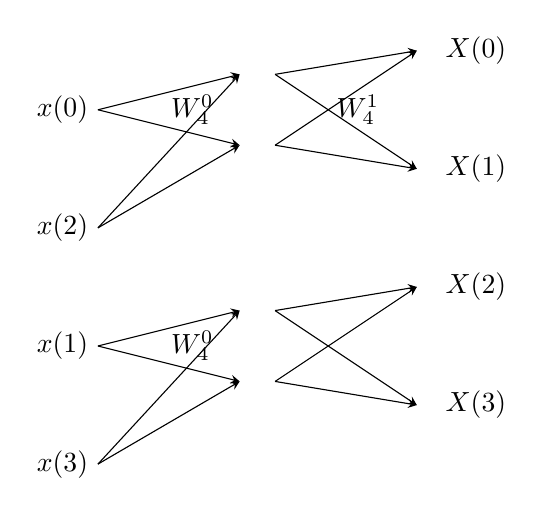
\begin{tikzpicture}[>=stealth,scale=1.5]
    % 输入节点
    \node at (0,4) {$x(0)$};
    \node at (0,3) {$x(2)$};
    \node at (0,2) {$x(1)$};
    \node at (0,1) {$x(3)$};

    % 第一级蝶形（W4^0）
    \draw[->] (0.3,4) -- (1.5,4.3);
    \draw[->] (0.3,3) -- (1.5,4.3);
    \draw[->] (0.3,4) -- (1.5,3.7);
    \draw[->] (0.3,3) -- (1.5,3.7);
    \node at (1.1,4.0) {$W_4^0$};

    \draw[->] (0.3,2) -- (1.5,2.3);
    \draw[->] (0.3,1) -- (1.5,2.3);
    \draw[->] (0.3,2) -- (1.5,1.7);
    \draw[->] (0.3,1) -- (1.5,1.7);
    \node at (1.1,2.0) {$W_4^0$};

    % 第二级蝶形（W4^0 和 W4^1）
    \draw[->] (1.8,4.3) -- (3.0,4.5);
    \draw[->] (1.8,3.7) -- (3.0,4.5);
    \draw[->] (1.8,4.3) -- (3.0,3.5);
    \draw[->] (1.8,3.7) -- (3.0,3.5);
    \node at (2.5,4.0) {$W_4^1$};

    \draw[->] (1.8,2.3) -- (3.0,2.5);
    \draw[->] (1.8,1.7) -- (3.0,2.5);
    \draw[->] (1.8,2.3) -- (3.0,1.5);
    \draw[->] (1.8,1.7) -- (3.0,1.5);

    % 输出节点
    \node at (3.5,4.5) {$X(0)$};
    \node at (3.5,3.5) {$X(1)$};
    \node at (3.5,2.5) {$X(2)$};
    \node at (3.5,1.5) {$X(3)$};
    \end{tikzpicture}
    \end{center}

    \textbf{计算复杂度分析：}
    直接 $N$ 点 DFT 的计算复杂度为 $\mathbf{O(N^2)}$；
    基‑2 FFT 算法的复杂度为 $\mathbf{O(N\log_2 N)}$。
    当序列长度 $N$ 增大时，直接 DFT 计算量呈平方级快速上升，而 FFT 仅以 $N\log_2 N$ 缓慢增长，长度越大，FFT 运算效率优势越明显。

\end{enumerate}

\vspace{1em}

%======================================================================
% 第5题 完整双方法解答
%======================================================================
\item 已知两有限长序列：
\[
x(n) = \cos\left(\frac{2\pi n}{N}\right)R_N(n),\quad h(n) = \sin\left(\frac{2\pi n}{N}\right)R_N(n)
\]
用直接卷积和 DFT 两种方法分别求以下的 $N$ 点圆周卷积：
\begin{enumerate}
    \item $y(n)=x(n)\circledast h(n)$；
    \item $y(n)=x(n)\circledast x(n)$；
    \item $y(n)=h(n)\circledast h(n)$。
\end{enumerate}

\textbf{解答：}

\textbf{方法一：DFT 方法（圆周卷积定理）}

圆周卷积定理：若 $y(n)=x(n)\circledast h(n)$，则
\[
Y(k) = N \cdot X(k)H(k)
\]
其中 $X(k)=\text{DFT}[x(n)]$，$H(k)=\text{DFT}[h(n)]$。

已知：
\[
X(k) = \frac{1}{2}\left[\delta(k-1)+\delta(k-N+1)\right]
\]
\[
H(k) = \frac{1}{2j}\left[\delta(k-1)-\delta(k-N+1)\right]
\]

\begin{enumerate}
    \item $y(n)=x(n)\circledast h(n)$
    \[
    Y(k) = N\cdot \frac{1}{2}\left[\delta(k-1)+\delta(k-N+1)\right] \cdot \frac{1}{2j}\left[\delta(k-1)-\delta(k-N+1)\right]
    \]
    \[
    Y(k) = \frac{N}{4j}\left[\delta(k-1)-\delta(k-N+1)\right]
    \]
    做 IDFT：
    \[
    y(n) = \frac{N}{2}\sin\left(\frac{2\pi n}{N}\right)R_N(n)
    \]

    \item $y(n)=x(n)\circledast x(n)$
    \[
    Y(k) = N\cdot \frac{1}{4}\left[\delta(k-1)+\delta(k-N+1)\right]^2
    \]
    \[
    Y(k) = \frac{N}{2}\delta(k) + \frac{N}{4}\left[\delta(k-1)+\delta(k-N+1)\right]
    \]
    做 IDFT：
    \[
    y(n) = \frac{N}{2}\delta(n) + \frac{N}{2}\cos\left(\frac{2\pi n}{N}\right)R_N(n)
    \]

    \item $y(n)=h(n)\circledast h(n)$
    \[
    Y(k) = N\cdot \frac{1}{-4}\left[\delta(k-1)-\delta(k-N+1)\right]^2
    \]
    \[
    Y(k) = \frac{N}{2}\delta(k) - \frac{N}{4}\left[\delta(k-1)+\delta(k-N+1)\right]
    \]
    做 IDFT：
    \[
    y(n) = \frac{N}{2}\delta(n) - \frac{N}{2}\cos\left(\frac{2\pi n}{N}\right)R_N(n)
    \]
\end{enumerate}

\textbf{方法二：直接卷积法（时域定义）}

$N$ 点圆周卷积定义：
\[
y(n) = \sum_{m=0}^{N-1}x(m)h((n-m))_N R_N(n)
\]
利用三角恒等式：
\[
\begin{aligned}
\cos A\sin B &= \frac{1}{2}[\sin(A+B)-\sin(A-B)] \\
\cos A\cos B &= \frac{1}{2}[\cos(A+B)+\cos(A-B)] \\
\sin A\sin B &= \frac{1}{2}[\cos(A-B)-\cos(A+B)]
\end{aligned}
\]
代入 $A=\frac{2\pi m}{N}, B=\frac{2\pi(n-m)}{N}$，并对 $m$ 求和，正交项求和为 0，可得：

\begin{enumerate}
    \item $y(n)=x(n)\circledast h(n)$
    \[
    y(n) = \frac{N}{2}\sin\left(\frac{2\pi n}{N}\right)R_N(n)
    \]

    \item $y(n)=x(n)\circledast x(n)$
    \[
    y(n) = \frac{N}{2}\delta(n) + \frac{N}{2}\cos\left(\frac{2\pi n}{N}\right)R_N(n)
    \]

    \item $y(n)=h(n)\circledast h(n)$
    \[
    y(n) = \frac{N}{2}\delta(n) - \frac{N}{2}\cos\left(\frac{2\pi n}{N}\right)R_N(n)
    \]
\end{enumerate}

两种方法结果一致，求解完毕。

\end{enumerate}
\section{第五次作业}

\subsection{1. 系统冲激响应与频率响应}
\noindent\textbf{原题：}
\begin{enumerate}[label=(\arabic*)]
    \item 已知微分方程 $\dfrac{\mathrm{d}}{\mathrm{d} t}y(t) + 3y(t) = 2\dfrac{\mathrm{d}}{\mathrm{d} t}x(t)$，求单位冲激响应 $h(t)$。
    \item 已知微分方程 $\dfrac{\mathrm{d}^2}{\mathrm{d} t^2}y(t) + \dfrac{\mathrm{d}}{\mathrm{d} t}y(t) + y(t) = \dfrac{\mathrm{d}}{\mathrm{d} t}x(t) + x(t)$，求单位冲激响应 $h(t)$。
    \item 因果LTI系统 $H(j\omega) = \dfrac{1}{j\omega+3}$，输出 $y(t)=e^{-3t}u(t)-e^{-4t}u(t)$，求输入 $x(t)$。
    \item 因果LTI系统差分方程 $y(n)-\dfrac{1}{6}y(n-1)-\dfrac{1}{6}y(n-2)=x(n)$，求频率响应 $H(\Omega)$ 和单位脉冲响应 $h(n)$。
\end{enumerate}

\subsubsection{解答}
\begin{enumerate}[label=(\arabic*)]
    \item
    对微分方程两边做傅里叶变换：
    \[
    j\omega Y(j\omega) + 3Y(j\omega) = 2j\omega X(j\omega)
    \]
    频率响应：
    \[
    H(j\omega) = \frac{Y(j\omega)}{X(j\omega)} = \frac{2j\omega}{j\omega+3} = 2 - \frac{6}{j\omega+3}
    \]
    逆变换得：
    \[
    h(t) = \boldsymbol{2\delta(t) - 6e^{-3t}u(t)}
    \]

    \item
    傅里叶变换：
    \[
    (j\omega)^2 Y + j\omega Y + Y = j\omega X + X
    \]
    \[
    H(j\omega) = \frac{j\omega+1}{(j\omega)^2+j\omega+1}
    \]
    极点 $s_{1,2}=\dfrac{-1\pm j\sqrt{3}}{2}$，部分分式展开后逆变换：
    \[
    h(t) = \boldsymbol{e^{-\frac{t}{2}} \left( \cos\frac{\sqrt{3}t}{2} + \frac{1}{\sqrt{3}}\sin\frac{\sqrt{3}t}{2} \right) u(t)}
    \]

    \item
    \[
    Y(j\omega) = \frac{1}{j\omega+3} - \frac{1}{j\omega+4}
    \]
    \[
    X(j\omega) = \frac{Y(j\omega)}{H(j\omega)} = \frac{1}{j\omega+4}
    \]
    \[
    x(t) = \boldsymbol{e^{-4t}u(t)}
    \]

    \item
    Z变换：
    \[
    H(z) = \frac{z^2}{z^2-\frac16 z-\frac16} = \frac{z^2}{\left(z-\frac12\right)\left(z+\frac13\right)}
    \]
    频率响应：
    \[
    H(\Omega) = \boldsymbol{\frac{e^{j2\Omega}}{\left(e^{j\Omega}-\frac12\right)\left(e^{j\Omega}+\frac13\right)}}
    \]
    部分分式展开：
    \[
    H(z) = \frac35\frac{z}{z-\frac12}+\frac25\frac{z}{z+\frac13}
    \]
    \[
    h(n) = \boldsymbol{\left[ \frac35\left(\frac12\right)^n + \frac25\left(-\frac13\right)^n \right] u(n)}
    \]
\end{enumerate}

\vspace{1em}
\hrule
\vspace{1em}

\subsection{2. 离散数据平均处理的频率响应}
\noindent\textbf{原题：}
$y(n)=\dfrac14\big[x(n)+x(n-1)+x(n-2)+x(n-3)\big]$，分别用时域、频域法求 $H(\Omega)$。

\subsubsection{解答}
\begin{enumerate}[label=(\arabic*)]
    \item \textbf{时域法}
    令 $x(n)=e^{j\Omega n}$：
    \[
    H(\Omega) = \frac14\left(1+e^{-j\Omega}+e^{-j2\Omega}+e^{-j3\Omega}\right)
    \]
    化简：
    \[
    H(\Omega) = \boldsymbol{\frac14 e^{-j\frac{3\Omega}{2}} \cdot \frac{\sin2\Omega}{\sin(\Omega/2)}}
    \]

    \item \textbf{频域法（Z变换）}
    \[
    H(z) = \frac14\left(1+z^{-1}+z^{-2}+z^{-3}\right)
    \]
    令 $z=e^{j\Omega}$：
    \[
    H(\Omega) = \boldsymbol{\frac14\left(1+e^{-j\Omega}+e^{-j2\Omega}+e^{-j3\Omega}\right)}
    \]
\end{enumerate}

\vspace{1em}
\hrule
\vspace{1em}

\subsection{3. 系统对周期信号的响应}
\noindent\textbf{原题：}
$H(j\omega)=\dfrac{1}{j\omega+1}$，$x(t)=\sin t+\sin3t$。
\begin{enumerate}[label=(\arabic*)]
    \item 求 $y(t)$；
    \item 说明波形变化；
    \item 写出无失真传输条件；
    \item 分析失真类型。
\end{enumerate}

\subsubsection{解答}
\begin{enumerate}[label=(\arabic*)]
    \item
    \[
    H(j1)=\frac{1-j}{2},\quad H(j3)=\frac{1-j3}{10}
    \]
    \[
    y(t) = \boldsymbol{\frac{\sqrt{2}}{2}\sin\left(t-\frac{\pi}{4}\right) + \frac{1}{\sqrt{10}}\sin\left(3t-\arctan3\right)}
    \]

    \item 高频分量幅度衰减更大，相位滞后更多，波形被平滑。

    \item 幅频：$|H(j\omega)|=K$；相频：$\angle H(j\omega)=-\omega t_0$。

    \item 存在 \textbf{幅度失真} 与 \textbf{相位失真}。
\end{enumerate}

\vspace{1em}
\hrule
\vspace{1em}

\subsection{4. 理想低通滤波器响应}
\noindent\textbf{原题：}
\[
H(\omega)=\begin{cases}
e^{-j\omega t_0},&|\omega|\le1\\
0,&|\omega|>1
\end{cases},\quad
x_1(t)=\frac{2\sin(t/2)}{t}
\]
\begin{enumerate}[label=(\arabic*)]
    \item 求 $x_2(t)=\left[x_1(t)-x_1(t-T)\right]*h(t)$；
    \item 证明对 $\pi\delta(t)$ 与 $\dfrac{\sin t}{t}$ 响应相同。
\end{enumerate}

\subsubsection{解答}
\begin{enumerate}[label=(\arabic*)]
    \item
    \[
    X_1(\omega)=2\pi\mathrm{rect}(\omega)
    \]
    \[
    x_2(t) = \boldsymbol{x_1(t-t_0)-x_1(t-t_0-T)}
    \]

    \item
    两者频谱在通带内均为常数 $\pi$，故输出相同：
    \[
    Y_a(\omega)=Y_b(\omega)=\pi e^{-j\omega t_0}
    \]
    因此响应相同。
\end{enumerate}

\vspace{1em}
\hrule
\vspace{1em}

\subsection{5. 滤波器设计}
\noindent\textbf{原题：}
设计巴特沃思低通：$\omega_p=1000\,\text{rad/s},\,A_p\le3\,\text{dB}$；$\omega_s=5000\,\text{rad/s},\,A_s\ge20\,\text{dB}$。
并分析 $H_a(s)=\dfrac{s}{s+a}$ 能否用冲激不变法。

\subsubsection{解答}
\begin{enumerate}[label=(\arabic*)]
    \item
    归一化 $\Omega_p=1,\Omega_s=5$，得阶数 $N=2$。
    \[
    H(s) = \boldsymbol{\frac{10^6}{s^2+1000\sqrt{2}\,s+10^6}}
    \]

    \item
    $H_a(s)$ 为高通滤波器，冲激不变法会产生 \textbf{频率混叠}，故不可用。
\end{enumerate}

\end{document}